\chapter{Requisitos Funcionais}

\section{Âmbito do projecto}

\subsection{Situação actual}

Escrever aqui situação actual do projecto!!

\begin{comment}
	Actualmente, o mercado financeiro de retalho oferece aos seus clientes uma grande variedade de simuladores de produtos de seguros, como os do ramo automóvel, motociclo, ciclomotor, saúde, habitação, etc. Aparte a simulação efectuada presencialmente com um Mediador, as várias Seguradoras oferecem uma interface \emph{Web} para a simulação dos seus produtos. No entanto, apenas conferem a opção de simular individualmente cada um dos produtos, não permitindo que seja efectuada uma simulação agregada de vários produtos oferecidos pela mesma Seguradora, com a possibilidade de se auferirem descontos em função de diversos factores como o perfil do utilizador, quantidade de produtos a contratar e o valor do prémio acumulado. Suprir esta lacuna é o mote para o desenvolvimento deste sistema de informação que deverá, paralelamente, permitir a configuração, validação e produção de simuladores para produtos financeiros.
\end{comment}


\subsection{Contexto do projecto}

Escrever aqui o contexto do projecto!!


\begin{comment}
	De forma a integrar melhor o sistema a desenvolver nas actividades quotidianas, é imperativo que se modele um diagrama de contexto, que clarifique quais as entidades externas ao sistema informático que vão ter algum relacionamento com este, isto é, quais as actividades que o sistema informático vai suportar no negócio em questão. Desta forma foram elaborados vários diagramas de contexto que visam clarificar essas actividades:
\end{comment}


\subsection{Diagrama de Contexto}

	\begin{figure}[!htb]
		\centering
		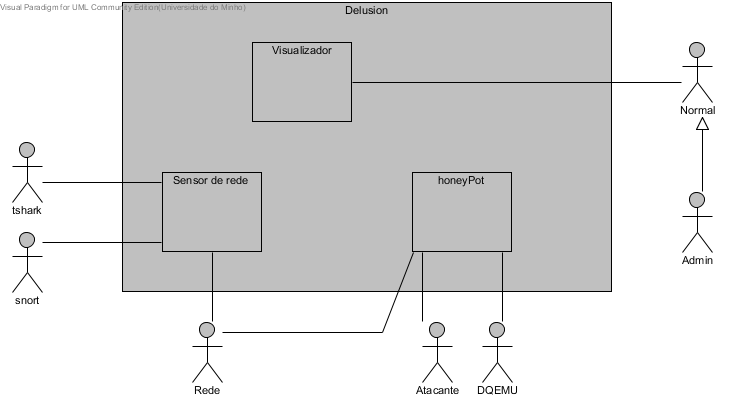
\includegraphics[scale=0.8]{images/DiagramaContexto}
		\caption{Diagrama de Contexto}
	\end{figure}


\pagebreak
